\documentclass{article}
\usepackage{times}
\documentclass{article}
\usepackage{amssymb}
\usepackage{amsmath}
\usepackage{graphicx} % Required for inserting images
\usepackage[a4paper, total={7in, 10in}]{geometry}

\title{Lista 2 - MAC0320}
\author{Paulo Henrique Albuquerque, NUSP $=12542251$ }
\date{}

\begin{document}

\maketitle

\textbf{E6.} 
\vspace{5mm}

\textbf{Solução.} 



\end{document}




\title{Sistemas de arquivos \\ {\large \color{red}Notas do capítulo 5}}

\newcommand\unix{{\color{red}UNIX} }
\newcommand\msdos{{\color{yellow}MS-DOS} }
\newcommand\winxp{{\color{blue}Windows XP} }
\newcommand\winnoveoito{{\color{pink}Windows 98} }
\newcommand\winnovecinco{{\color{green}Windows 95} }

\begin{document}

\maketitle

\section{Introdução aos arquivos}
Os três requisitos para armazenamento de informação a longo prazo são:

\begin{itemize}
  \item deve ser possível armazenar uma grande quantidade de informação.
  \item a informação deve sobreviver à terminação do processo que a usa. 
  \item múltiplos processos devem ser capazes de acessar a informação de forma concorrente.
\end{itemize}

A solução usual para todos esses problemas é armazenar informação em discos em unidades chamadas \textbf{arquivos}. A informação presente nessas unidades precisa ser \textbf{persistente}, ou seja, não deve ser afetada pela criação ou terminação de processos.

Arquivos são gerenciados pelo sistema operacional. A parte do SO responsável por esse gerenciamento é conhecido como o \textbf{sistema de arquivos}.

\subsection{Arquivos}

\subsubsection{Nomes de arquivos}
Arquivos são abstrações. Eles são uma forma de armazenar informação em disco para ser lida depois. Isso deve ser feito de forma que o usuário não precise se preocupar com os detalhes de como a informação é armazenada e como discos funcionam. Uma das características mais importantes de um \textit{mecanismo de abstração} é como os objetos são nomeados. Examinemos como arquivos são nomeados nos diferentes sistemas de arquivos.
No sistema \unix, há distinção entre letras maíusculas e minúsculas, \msdos não faz essa distinção.

O sistema \winxp tem um sistema nativo, o New Technology File System (NTFS) que suporta nomes de arquivos em Unicode. 

Em alguns sistemas, como \unix, extenções não são forçadas. O Windows é bastante ciente das extensões dos arquivos e atribui significado para as diferentes extensões. Algo estranho nesse sistema é que, apesar das extensões serem importantes, elas são escondidas por padrão. Isso pode ser alterado pelo usuário.

\subsubsection{Estrutura dos arquivos}
Há três formas comuns para estruturar arquivos:
\begin{itemize}

    \item arquivo como uma simples sequência de bytes. Esse é o jeito \unix e \winnoveoito. O sistema não se importa com o que está no arquivo, tudo que vê são bytes. Qualquer significado é imposto por programas de usuário.  
  \item arquivo como sequência de registros de tamanhos fixos. Cada registro tem um estrutura interna. As operações de leitura e escrita atuam sobre registros.
  \item arquivo como um árvore de registros. Cada registro tem um chave, que é usada para buscas rápidas. É amplamente utilizado em mainframes ainda utilizados em grandes centros de processamento de dados.

\end{itemize}

\begin{figure}[h!]
  \begin{center}
    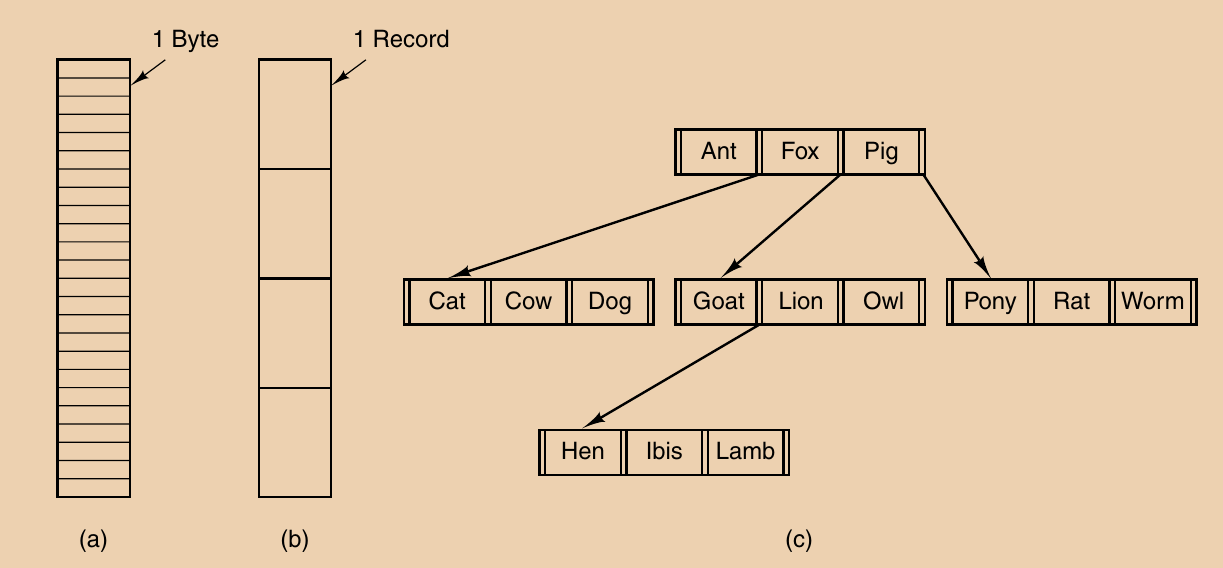
\includegraphics[width=0.45\textwidth]{img/5-2.png}
  \end{center}
  \caption{Tipos de estruturas para arquivos}
  \label{fig:}
\end{figure}

\subsubsection{Tipos de arquivos}
Há vários tipos de arquivos definidos em diferentes SOs. O \unix define \textbf{arquivos regulares e diretórios}, além de definir arquivos especiais, de bloco e de caracteres. No \winxp há arquivos de \textbf{metadados}.


\textbf{Arquivos regulares} contém informações de usuário. \textbf{Diretórios} são arquivos de sistema que mantêm a estrutura do sistema de arquivos. \textbf{Arquivos de caracteres} estão relacionados a dispositivos I/O. \textbf{Arquivos de bloco} são usados para modelar discos. Estamos interessados aqui em arquivos regulares e de diretórios, principalmente.

Em geral, arquivos regulares são arquivos texto (ASCII) ou arquivos binários. Arquivos binários têm uma esrtutura interna conhecida pelos programas que os usam. 
Um exemplo de arquivo binário é um arquivo executável do \unix ou um arquivo "archive", também do \unix. Eles são mostrados na figura abaixo.

\begin{figure}[h]
  \begin{center}
    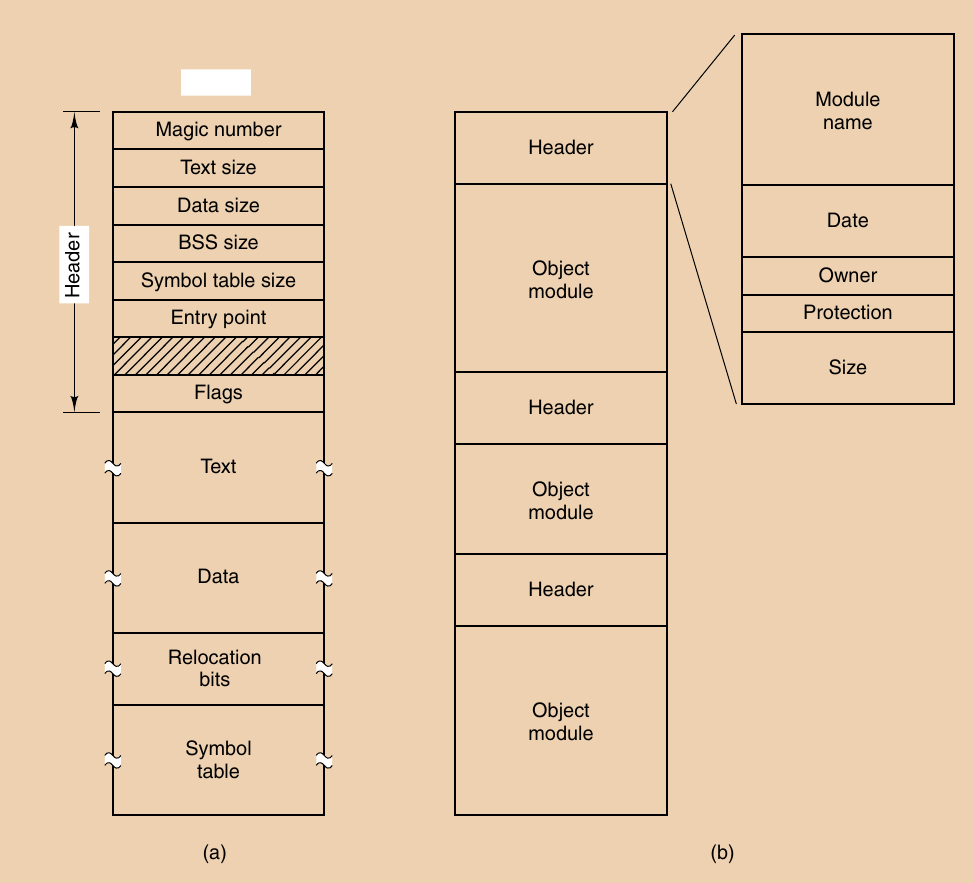
\includegraphics[width=0.45\textwidth]{img/5-3.png}
  \end{center}
  \caption{}
  \label{fig:}
\end{figure}

Apesar do SO enxergar um arquivo executável apenas como uma sequência de bytes, ele somente irá executá-lo se o arquivo tiver um formato adequado. Por exemplo, na seção "header" de um executável do \unix, o campo \textbf{magic number} identifica o arquivo como executável: arquivos que não têm essa flag ativada não serão executados pelo SO. Seguido do header, há o segmento de texto e de dados do programa. Eles são carregados na memória.

\subsubsection{Acesso de arquivos}

Há dois tipos comuns de acesso a arquivos, sequencial e aleatório. Sistemas antigos só forneciam o primeiro. Nesse tipo de acesso, um processo deve ler os bytes de um arquivo em ordem. Quando discos são utilizados para armazenar arquivos, é possível ler bytes fora de ordem. Arquivos que podem ser acessados fora de ordem são chamados de \textbf{arquivos de acesso aleatório}. Eles são necessários para várias aplicações. Por exemplo, se um cliente de uma companhia aérea deseja reservear uma vaga em um voo, o programa que faz a reserva deve ser capaz de acessar o arquivo de reservas desse vôo sem ter que ler os arquivos de milhares de outros vôos. 

Há dois métodos para especificar onde começar a ler o arquivo. No primeiro, toda operação \verb|read| dá a posição no arquivo onde começa a leitura. No segundo, a chamada \verb|seek| é feita para configurar a posição corrente de leitura. Depois dessa chamada, o arquivo pode ser lido sequencialmente. 

Sistemas operacionais modernos consideram todos os arquivos como de acesso aleatório.

\subsubsection{Atributos de arquivos}

Todo arquivo tem um nome e seus dados. Em adição a isso, todos sistemas operacionais associam outras informações a cada arquivo, por exemplo, a data de criação do arquivo. Essas informações adicionais são chamadas de \textbf{atributos} do arquivo. Algumas pessoas chamam de \textbf{meta dados}. A lista de atributos depende da implemnetação de cada sistema operacional.

Alguns atributos possíveis são mostrados abaixo.

\begin{figure}[h]
  \begin{center}
    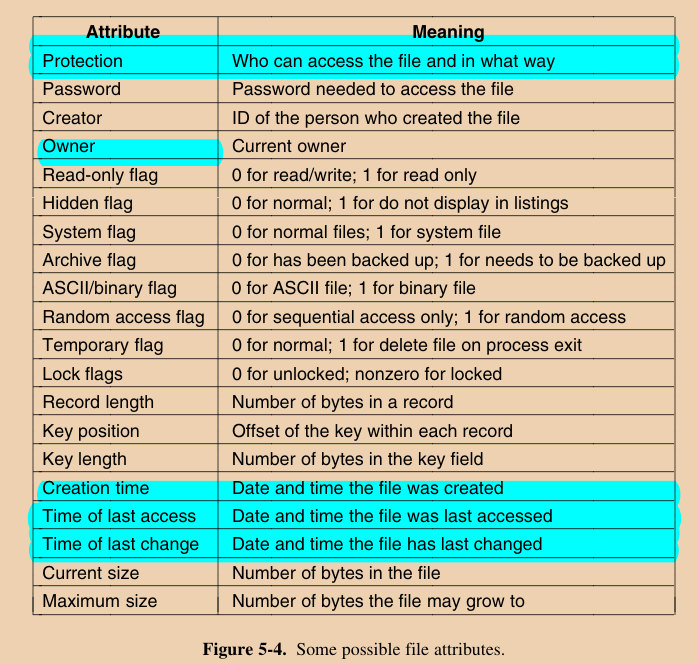
\includegraphics[width=0.45\textwidth]{img/5-4.png}
  \end{center}
  \caption{}
  \label{fig:}
\end{figure}

Os vários atributos de "tempo" marcam quando o arquivo foi criado, tempo do último acesso e tempo de última modificação. Esses atributos são úteis para vários programas. Por exemplo, um código fonte modificado desde a última compilação deve ser compilado novamente.

\subsection{Operações}

Abaixo listamos as operações possíveis em arquivos, juto com uma breve descrição.

\begin{itemize}
  \item Create. O arquivo é criado sem nenhum dado. O objetivo dessa call é avisar ao SO que um arquivo foi criado e assim ele pode configurar alguns atributos.
  \item Delete. Deleta o arquivo para liberar espaço no disco.
  \item Open. Antes de usar um arquivo, ele precisa ser aberto. O propósito dessa chamada é permitir que o SO traga os atributos e lista de endereços de blocos de discos do arquivo para memória para acessos futuros rápidos.
  \item Close. O arquivo é liberado para liberar memória.
  \item Read. Lê dados do arquivo. A chamada deve especificar a quantidade de bytes que deseja ler e um buffer para armazená-los.
  \item Write. Escreve no arquivo.
  \item Append. Escreve no final do arquivo.
  \item Seek. Reposiciona o ponteiro de arquivo para leitura ou escrita. 
  \item Get attributes.
  \item Set attributes.
  \item Rename.
  \item Lock. Proibe acesso simultâneo por diferentes processos.
\end{itemize}

\section{Diretórios}
São utilizados para manter a estrutura do sistema de arquivos. Em muitos sistemas, são arquivos.

\subsection{Diretórios simples}
Um diretório simples contém um número de entradas, uma por arquivo.

Quando um arquivo é aberto, o SO procura seu diretório até achar o nome do arquivo a ser aberto. Após encontrar, extrai os atributos e endereços de discos da entrada do diretório ou da estrutura de dados apontada por ela, e coloca esses dados na memória. Todas referências futuras ao arquivo são feitas usando essas informações na memória.

O número de diretórios varia de sistema para sistema. A forma mais simples é um único diretório contendo todos os arquivos de todos os usuários. Isso é problemático em situações em que múltiplos usuários usam nomes de arquivos iguais: nesse cenário, o sistema não consegue distinguir os dois arquivos quando uma chamada Open é feita, por exemplo. 

Uma possível solução para isso é utilizar diferentes diretórios para diferentes usuários. Isso permite nomes iguais de arquivos para diferentes usuários.

Outra melhora possível é permitir que um mesmo usuário tenha vários diretórios, para propósitos de organização. Isso é uma \textbf{hierarquia geral}, ou seja, uma árvore de diretórios. Veja a figura abaixo.

\begin{figure}[h]
  \begin{center}
    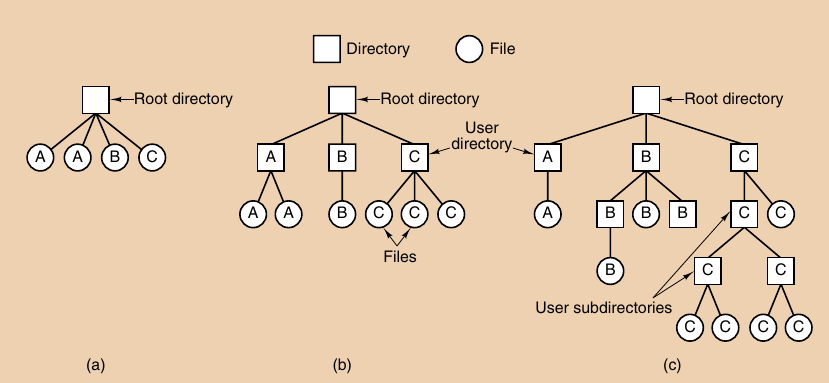
\includegraphics[width=0.45\textwidth]{img/5-6.png}
  \end{center}
  \caption{}
  \label{fig:}
\end{figure}

Pelo grande poder de organização oferecido por essa última estrutura de diretório, quase todos sistemas de arquivos modernos a utilizam.

\subsection{Caminhos}

Dois métodos são utilizados para especificar o caminho de arquivos na árvore: \textbf{caminhos absolutos} e \textbf{caminhos relativos}. Caminhos absolutos começam com "/" (No \unix) e consistem de um caminho a partir da raiz da árvore de diretórios (root). Caminhos relativos são caminhos relativos ao diretório corrente (working directory "pwd"). O diretório corrente é um conceito utilizado para que processos possam especificar a partir de onde caminhos relativos devem começar. Cada processo tem seu próprio diretório corrente.

No \unix e na maioria dos sistemas modernos, cada diretório faz referência a si mesmo com "." e ao seu pai na árvore com "..".

\subsection{Operações em diretórios}

\begin{itemize}
  \item Create. Um diretório é criado vazio com exceção do "." e "..".
  \item Delete. Somente diretórios vazios podem ser deletados do sistema de arquivos. Um diretório apenas com "." e ".." é considerado vazio.
  \item Opendir.
  \item Closedir.
  \item Readdir.
  \item Rename.
  \item Link.
  \item Unlink.
\end{itemize}

\section{Implementação de Sistemas de Arquivos}

Agora analisemos o lado do implementador de sistemas de arquivos. Eles estão interessados em como arquivos e diretórios são armazenados, como espaço de disco é gerenciado e como fazer tudo funcionar eficientemente.

\subsection{Layout}
Sistemas de arquivos são geralmente armazenados em discos.

A maioria dos discos podem ser divididos em partições, com sistemas de arquivos independentes. O setor 0 do disco é chamado de \textbf{MBR} (Master Boot Record) e é usado para o boot. O final do MBR contém a tabela de partições, que dá os começos e finais de cada partição. Uma partição é marcada como ativa. Quando o computador é iniciado, a BIOS lê e executa o código no MBR. A primeira coisa que o programa no MBR faz é localizar a partição ativa, lê seu primeiro bloco, chamado \textbf{bloco de boot} e o executa. Esse código carrega o sistema operacional contido naquela partição. Toda partição contém um bloco de boot, mesmo que não contenha nenhuma SO. A descrição acima deve ser respeitada para todo hardware que utiliza BIOS para inicializar sistemas operacionais. 
 
Vale ressaltar que alguns sistemas não exigem uma partição ativa: eles fornecem um menu para que o usuário escolha uma partição para boot. 

O layout de partição varia de sistema para sistema. Para sistemas baseados no \unix, o sistema de arquivo contém alguns dos itens mostrados na figura abaixo. Abaixo mostramos uma possível ordem de seções na partição.

\begin{figure}[h]
  \begin{center}
    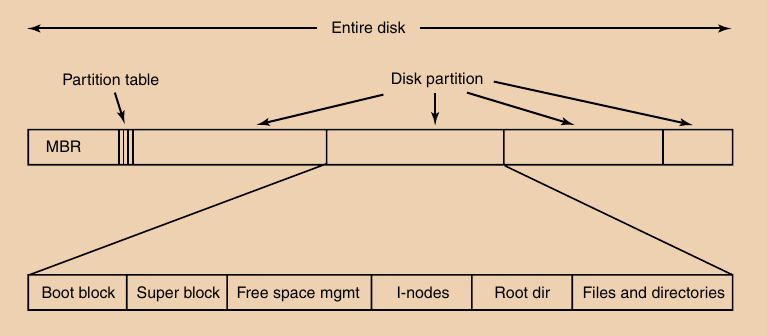
\includegraphics[width=0.45\textwidth]{img/5-8.png}
  \end{center}
  \caption{}
  \label{fig:}
\end{figure}


\begin{itemize}
  \item 1. Superblock. Contém todos os atributos principais do sistema de arquivos e é levado para a memória quando o computador é inicializado.
  \item 2. Blocos livres.
  \item 3. I-nodes. Estrutura de dados que diz tudo sobre cada arquivo e aonde estão localizados seus blocos.
  \item 4. Diretório root.
  \item 5. Todo o restante dos arquivos e diretórios.
\end{itemize}

\subsection{Implementando arquivos}

A questão mais importante sobre implementação de arquivos é guardar os blocos correspondentes a cada arquivo.

\subsubsection{Alocação contínua}

O esquema mais simplório é armazenar cada arquivo como uma sequência contínua de blocos de disco. Isso é suficientemente simples pois basta guardamos o endereço do primeiro bloco do arquivo e a quantidade de blocos no arquivo. Esse esquema também é eficiente porque um arquivo pode ser lido apenas com um \verb|read|. Apenas um \verb|read| é necessário (para o primeiro bloco do arquivo).

Um grande problema desse esquema é que, com o tempo o disco torna-se fragmentado, e quando o disco enche, é necessário fazer uma compactação, o que é muito custoso. Outra alternativa é reutilizar blocos livres. Isso é possível mantendo uma lista de blocos livre. A princípio isso é factível. Porém, quando um novo arquivo for criado é necessário especificar o tamanho final do arquivo, o que não é possível na maioria dos cenários.

Hoje em dia, há alguns usos de alocação contínua: CD-ROM's e DVD's.

\subsubsection{Listas ligadas}

Uma segunda alternativa para armazenar arquivos é manter uma lista ligadas dos blocos utilizados por cada arquivo. A primeira palavra de cada bloco é usada como ponteiro para o próximo bloco da lista, o restante do bloco é utilizado para dados.

\begin{figure}[h]
  \begin{center}
    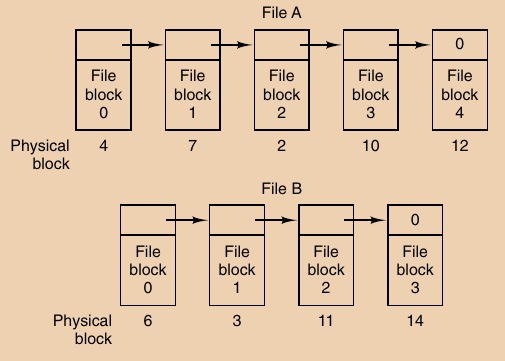
\includegraphics[width=0.45\textwidth]{img/5-9.png}
  \end{center}
  \caption{}
  \label{fig:}
\end{figure}

Todos os blocos do disco podem ser utilizados nesse esquema. Nenhum espaço é perdido devido a fragmentação. Além disso, é suficiente para a entrada no diretório desse arquivo somente armazenar o endereço para o primeiro bloco: o restante pode ser encontrado a partir daí. 

Ler um arquivo sequencialmente é fácil: para ler $n$ bytes consecutivos, são feitas $n$ leituras de blocos. Cada leitura dá um "pedaço" dos dados e o endereço do próximo bloco que deve ser lido. Já para acesso aleatório o processo é ineficiente. Para acessar o $n$-ésimo bloco, o sistema precisa ler os $n-1$ blocos anteriores, para saber qual o endereço do $n$-ésimo bloco. Outro ponto negativo desse esquema é que a quantidade de dados num bloco não é potência de dois, por causa do espaço necessário para os ponteiros. Alguns programas leêm e escrevem em blocos cujo tamanho é potência de dois. Além disso, nesse esquema é necessário concatenar informações de discos, o que gera overhead devido a cópia.

\subsubsection{Listas ligadas usando tabela em memória}

Ambas desvantagens do esquema anterior podem ser resolvidas ao colocar todas as palavras referentes ao ponteiros numa tabela em memória. Uma tabela desse tipo é chamada \textbf{FAT (File Allocation Table)}.

\begin{figure}[h]
  \begin{center}
    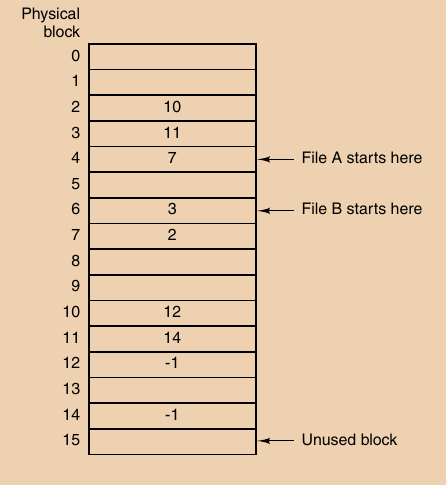
\includegraphics[width=0.45\textwidth]{img/5-10.png}
  \end{center}
  \caption{}
  \label{fig:}
\end{figure}

Usando essa organização, todo o bloco fica disponível para dados. Além disso, acesso aleatório é simples, pois podemos encontrar o endereço do bloco inicial (referente ao offset desejado) apenas utilizando as informações na memória, o que é bem mais rápido do que "seguir ponteiros" fazendo leituras no disco. As entradas de diretório dos arquivos devem guardar somente o endereço do bloco inicial.

A desvantagem principal desse método é que a tabela inteira deve estar na memória a todo tempo.

\subsubsection{I-Nodes}

O último método é associar cada arquivo a uma estrutura de dados chamada de \textbf{i-node} (\textbf{index-node}), que lista os atributos e endereços de disco dos blocos do arquivo. A grande vantagem desse esquema em relação aos esquemas anteriores é que somente o i-node do arquivo a ser aberto precisa estar na memória.

Um problema que surge com i-nodes é que cada arquivo tem uma quantidade fixa de referências à endereços de disco, mas o arquivo pode crescer indefinidamente. Nesses casos, uma solução é reservar o último endereço de disco não para um bloco de dados, e sim para um \textbf{bloco indireto} que faz referências para outros endereços de blocos. Essa ideia pode ser extendida para \textbf{blocos indiretos duplos} e \textbf{blocos indiretos triplos}, como mostrado na figura abaixo.

\begin{figure}[h]
  \begin{center}
    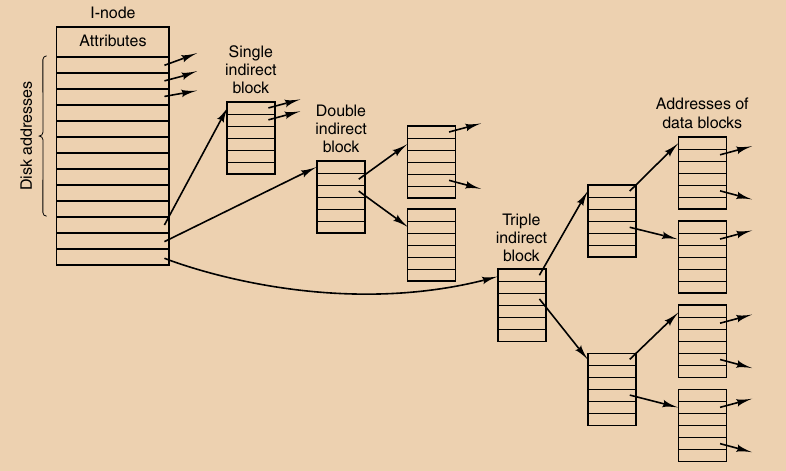
\includegraphics[width=0.45\textwidth]{img/5-11.png}
  \end{center}
  \caption{}
  \label{fig:}
\end{figure}

\subsection{Implementando diretórios}

Para que o sistema leia um arquivo ele precisa ser aberto, e para ele ser aberto ele precisa ser primeiramente achado a partir do caminho fornecido pelo usuário. O primeiro passo é localizar o diretório root. Esse diretório pode estar numa posição fixa relativa ao início de uma partição. Alternativamente, sua posição pode ser determinada \textit{a partir de outras informações}. Por exemplo, em um sistema clássico \unix, o superblock contém informação sobre o tamanho das estruturas de dados que precedem a área de dados. Ou seja, a área de "Free space mgmt" no diagrama da partição de um sistema de arquivos \unix. Então, podemos identificar o começo dos i-nodes. O primeiro i-node é o da raiz (ele é criado quando o sistema de arquivos é criado). No \winxp, a informação no setor de soot localiza a \textbf{MFT (Master File Table)}, que é usada para localizar outras partes do sistema de arquivos.

Localizada a raiz, uma busca na árvore é feita para encontrar a entrada de diretório do arquivo requerido. Ela contém as informações necessárias para acessar os blocos do arquivo. Em qualquer caso de esquema, o objetivo principal do sistema de diretórios é mapear nomes de arquivos em ASCII para as informações necessárias para localizar os dados.

Agora, surge a pergunta: onde armazenar os atributos de um arquivo? Uma possibilidade óbvia é armazenar diretamente na entrada do diretório. Nesse caso, a entrada do diretório contém o nome do arquivo, uma estrutura que armazena os atributos e um ou mais endereços de disco, que dizem onde os blocos estão. Tudo com tamanhos pré-definidos.

Para sistemas que usam i-nodes, outra possibilidade é armazenar os atributos nos próprios i-nodes. Nesse caso, a entrada do diretório de um arquivo contém somente o nome do arquivo e o número do i-node correspondente.

\subsubsection{Arquivos compartilhados}

Veja a figura abaixo, que mostra um arquivo compartilhado entre dois diretórios distintos.

\begin{figure}[h]
  \begin{center}
    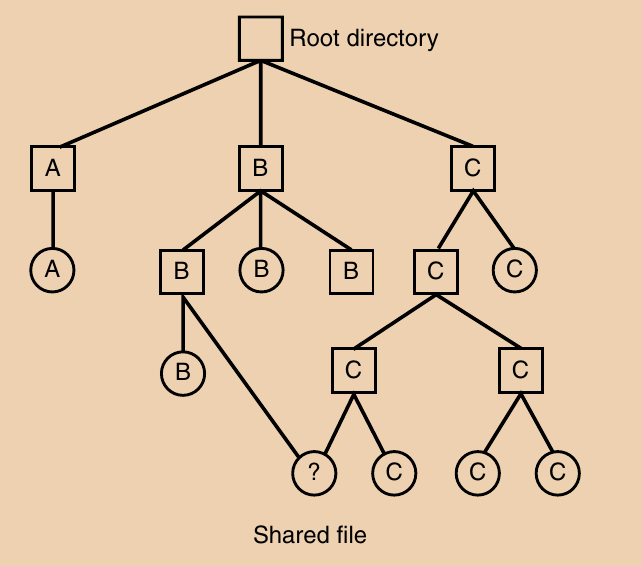
\includegraphics[width=0.45\textwidth]{img/5-12.png}
  \end{center}
  \caption{}
  \label{fig:}
\end{figure}

No \unix, o uso de i-nodes para armazenar atributos de arquivos faz com que compartilhamento de arquivos seja simples: qualquer número de diretórios pode apontar para um único i-node.

O i-node contém um campo que é incrementado quando um novo link é adicionado, e é decrementado quando um link é removido. Somente quando o contador chega a zero os dados e o i-node são deletados.

Esse tipo de link é chamado de \textbf{link físico}. Esse tipo de link tem duas "fraquezas". A primeira é que links só podem ser feitos dentro de um mesmo sistema de arquivos (partição). A outra é que a um i-node está associado somente um conjunto de atributos. Então, em uma situação em que há compartilhamento de um arquivo, o dono do arquivo pode deletar a sua entrada do diretório e outros usuários que apontam para esse arquivo ficaram impossibilitados de modificá-lo ou deletá-lo, pois os atributos dele ainda apontam o usuário original como dono do arquivo.

Há outra forma de compartilhar arquivos. Nela, cria-se um arquivo cujos "dados" é um caminho para outro arquivo. Esse tipo de link funciona através de diferentes sistemas de arquivos. Esse tipo de link é chamado de \textbf{link simbólico} em sistemas \unix, \textbf{atalho} em sistemas Windows e um \textbf{alias} no MAC OS. Links simbólicos podem ser usados em sistemas que armazenam atributos dentro da entrada do diretório. É difícil sincronizar diferentes diretórios contendo diferentes atributos para esse arquivo: uma mudança no arquivo deve afetar toda entrada de diretório apontando para esse arquivo. Mas as entradas de diretório extras não contêm os atributos desse arquivo, por isso a dificuldade. Outro problema é que quando um arquivo é deletado, links para ele se tornam orfãos.

As sutilezas desses tipos de links podem ser observadas abrindo um terminal no UNIX e testando remoções e modificações (bom exercício).

Agora, vemos algumas implementações de diretórios em diferentes sistemas.

\subsubsection{Diretórios no \winnoveoito}

O sistema de arquivos do release original do \winnovecinco era idêntico ao sistema de arquivos do \msdos, mas um novo release adicionou suporte para nomes de arquivos mais longos e arquivos maiores. Esse novo release é referido como o sistema de arquivos do \winnoveoito, apesar de ser encontrado em alguns sistemas \winnovecinco.

Há dois tipos de diretórios no \winnoveoito. O mostrado abaixo chamamos de \textbf{base entry}.

\begin{figure}[h]
  \begin{center}
    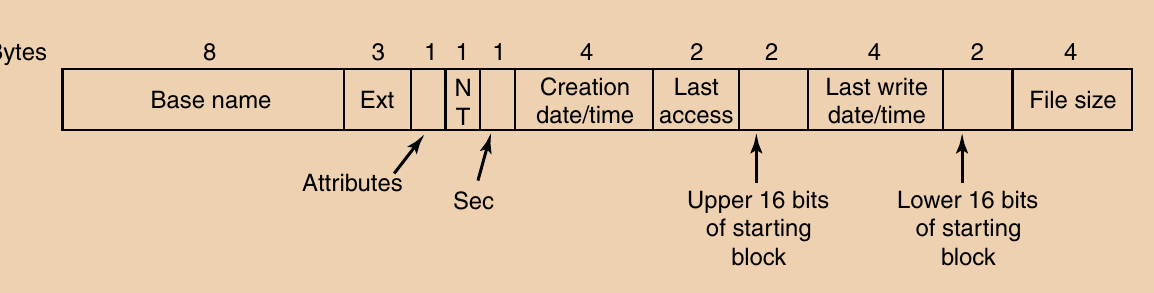
\includegraphics[width=0.45\textwidth]{img/5-13.png}
  \end{center}
  \caption{}
  \label{fig:}
\end{figure}

Essa entrada de diretório "base" contém todas as informações contidas em versões passadas do Windows e mais. O upgrade mais importante foi o aumento de bits para o campo que aponta para o primeiro bloco de 16 para 32. Isso aumentou o sistema de arquivos de $2^{16}$ blocos para $2^{32}$ blocos, o que é um aumento grande.

Essa estrutura provém apenas para o antigo estilo de nome de arquivos 8 + 3 caracteres herdado do \msdos. E nomes de arquivos longos? A resposta para esse problema enquanto mantém a retro-compatibilidade com sistemas passados é usar entradas de diretório adicionais. A figura abaixo mostra outro tipo de entrada de diretório, que pode conter até 13 caracteres de um nome de arquivo longo. Um arquivo pode estar associado a várias entradas desse tipo. Elas são colocadas antes da entrada "base" em ordem reversa. O campo "Attributes" de cada entrada de nome longo contém o valor 0xF, que é impossível para sistemas de arquivos de SO's antigos (\msdos e \winnovecinco). Então essas entradas são ignoradas em sistemas antigos. O campo "Sequence" diz ao sistema qual é a última entrada. 

Se isso parece uma confusão é porque é: prover retro-compatibilidade enquanto adiciona novas funcionalidades para um sistema novo geralmente gera uma bagunça.

\subsubsection{Diretórios no \unix}

A estrutura tradicional de um diretório \unix é extremamete simples. Cada entrada contém um nome de arquivo e o número do seu i-node. Todas as informações adicionais do arquivo estão no i-node. 

\begin{figure}[h]
  \begin{center}
    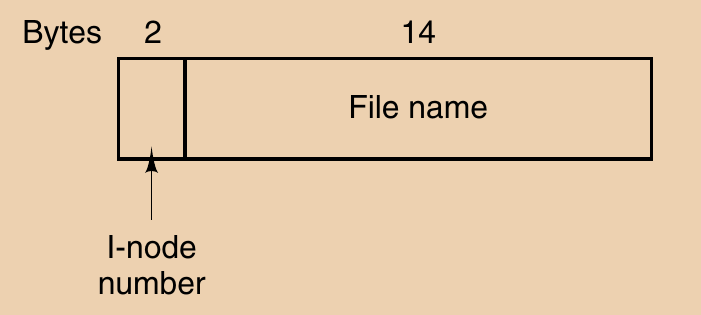
\includegraphics[width=0.45\textwidth]{img/5-15.png}
  \end{center}
  \caption{}
  \label{fig:}
\end{figure}

Quando um arquivo é aberto, o sistema deve achar os blocos do arquivo. Primeiro o sistema localiza a raiz da árvore do sistema de arquivos. Os i-nodes formam um simples array que são localizados usando as informações do superbloco. A primeira entrada do array é o i-node do root. Após localizar o i-node do root, o sistema lê o conteúdo do diretório root, que dára o i-node do próximo diretório, e assim por diante. 

\begin{figure}[h]
  \begin{center}
    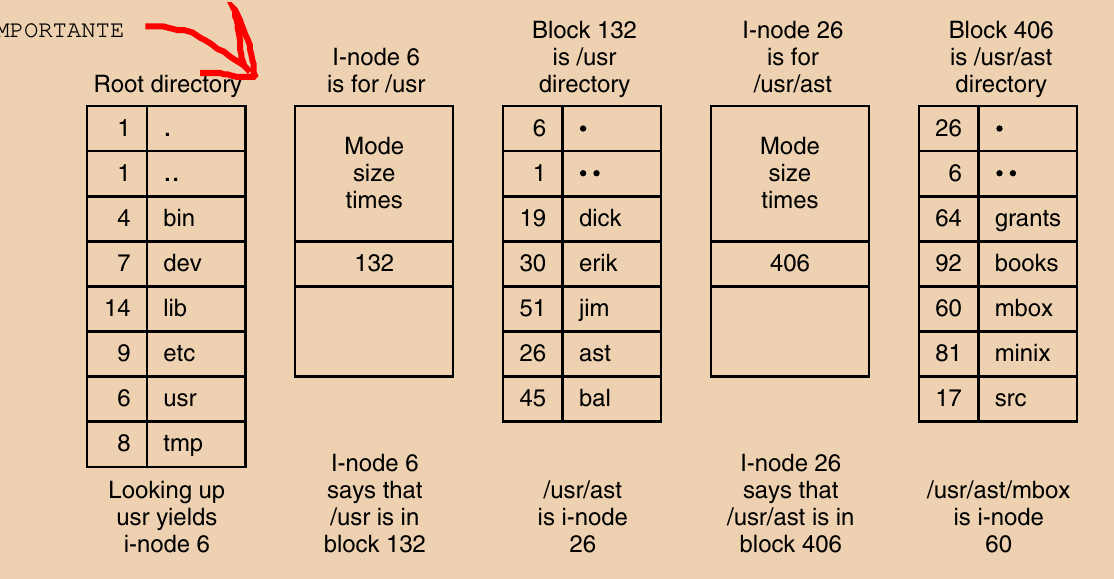
\includegraphics[width=0.45\textwidth]{img/5-16.png}
  \end{center}
  \caption{}
  \label{fig:}
\end{figure}

Caminhos relativos são localizados da mesma forma que caminhos absolutos, só que começando no diretório corrente do processo. Nenhum mecanismo especial é utilizado para tratar os diretórios "." e "..": para o sistema de arquivos, eles são só strings ASCII ordinárias e são tratadas da mesma forma que os outros nomes.

\subsubsection{Diretórios no NTFS}

O sistema \textbf{NTFS} (\textbf{New Technology File System}) da Microsoft é o sistema de arquivos padrão. Ele provém múltiplos conjuntos de caracteres ao usar Unicode para nome de arquivos. Mas usar múltiplas linguagens faz surgirem alguns problemas. Por exemplo, algumas línguas têm formas de ordenação lexicográfica distintas. A solução é ter um atributo somente para convenções de linguagem para a língua do arquivo em questão. "Mais atributos" é a solução NTFS para vários problemas. 

No \unix, um arquivo é somente uma sequência de bytes. No NTFS, um arquivo é uma coleção de atributos, e cada atributo é uma stream de bytes. A estrutura de dados básica é a \textbf{MFT} (\textbf{Master File Table}) que fornece 16 atributos, onde cada um pode ter 1 KB. Um atributo dentro da MFT pode ser um ponteiro para um arquivo adicional se necessário. 

Os dados no NTFS são armazenados em um atributo. Um arquivo NTFS pode ter mais de uma stream de dados. Múltiplas streams de dados podem ter vários usos. Por exemplo, uma imagem grande pode ter uma pequena thumbnail associada a ela, e essas duas imagens podem ser armazenadas em streams diferentes de dados. No outro extremo, NTFS pode lidar com arquivos pequenos colocando centenas de bytes no atributo header. Isso é chamado de uma \textbf{arquivo imediato} (Mullender and Tanenbaum, 1984).

\subsubsection{Gerenciamento de espaço em disco}

Arquivos são normalmente armazenados em discos. Evidentemente, gerenciamento de espaço de disco é uma grande preocupação para os implementadores de sistemas. Conforme vimos, há duas formas principais de armazenar um arquivo de $n$ bytes: usando $n$ bytes consecutivos no discos ou usando um número de blocos não necessariamente consecutivos. Armazenar de forma consecutiva tem a desvantagem de, que se um arquivo cresce, provavelmente terá de ser movido no disco, o que é bastante custoso. Por essa razão, quase todos os sistemas "cortam" o arquivo em blocos de tamanho fixado que não são adjacentes no disco.

\subsubsection{Tamanho do bloco}

Naturalmente, surge a pergunta: qual tamanho de bloco utilizar? Utilizar conhecimentos sobre a estrutura interna do disco é claramente uma forma de tomar essa decisão. Porém, isso é altamente dependente do dispositivo, o que é uma grande desvantagem. 

Um tamanho grande demais de bloco faz com que arquivos pequenos utilizem um cilindro inteiro, por exemplo. Tamanhos pequenos demais, fazem com que cada arquivo consiste em um grande número de blocos. Ler cada bloco normalmente requer um \textit{seek} e um \textit{rotational delay} o que torna a leitura de todos esses blocos lenta.

Para decidir o tamanho, observe os seguintes fatos. O tempo de acesso de um bloco é completamente dominado pelo tempo de seek e rotational delay. Então, quanto mais dado é trazido do disco, melhor. Ou seja, a taxa de transferência de dados aumenta com o tamanho do bloco. 

Por outro lado, usar tamanhos de blocos pequenos que são potências de dois maximizam o uso de disco. A medido que o tamanho do bloco cresce, algum espaço é desperdiçado: poucos discos são múltiplos do tamanho do disco e provavelemente é desperdiçado espaço no último bloco do arquivo.

Portanto, espaço e performance são inerentemente conflitantes. Um tamanho "in-between" deve ser escolhido. Para sistemas \unix, o tamanho 1KB é utilizado. Para o \msdos, o tamanho do bloco pode ser qualquer potência de dois entre 512 bytes e 32KB. Isso é determinado olhando para o tamanho do disco e outras razões não relacionadas aos argumentos dados acima.

\subsubsection{Gerenciando blocos livres}

Agora que o tamanho dos blocos foi discutido, uma questão é como gerenciar os blocos livres. Dois métodos são comumente utilizados. O primeiro consiste em usar uma lista ligada de blocos, onde cada bloco guarda quantos blocos livres possíveis conseguir. Evidentemente alguns bytes são necessários para apontar para o próximo bloco da lista. Geralmente, blocos livres são utilizados para armazenar a lista. 

Outra forma é manter um bitmap. Um disco com $n$ blocos precisa de um bitmap de $n$ bits. Blocos livres são representados por 1s e blocos alocados por 0s (ou vice versa, obviamente). Esse tipo de armazenamento de blocos livres requer menos espaço em geral, visto que cada bloco livre precisa de somente um bit, em vez de 32 na representação por lista ligada. Somente quando o disco está quase totalmente alocado é que a lista ligada ocupa menos espaço. Porém, a lista ligada tem a vantagem que somente um bloco de ponteiros precisa estar na memória. Quando um arquivo é criado, os blocos necessários são obtidos por esse bloco de ponteiros. Se precisar de mais blocos, outro bloco de ponteiros é lido do disco. Similarmente, quando um arquivo é deletado, seus blocos são livrados e adicionados ao bloco de ponteiros na memória. Quando esse bloco enche, é escrito no disco.

\begin{figure}[h]
  \begin{center}
    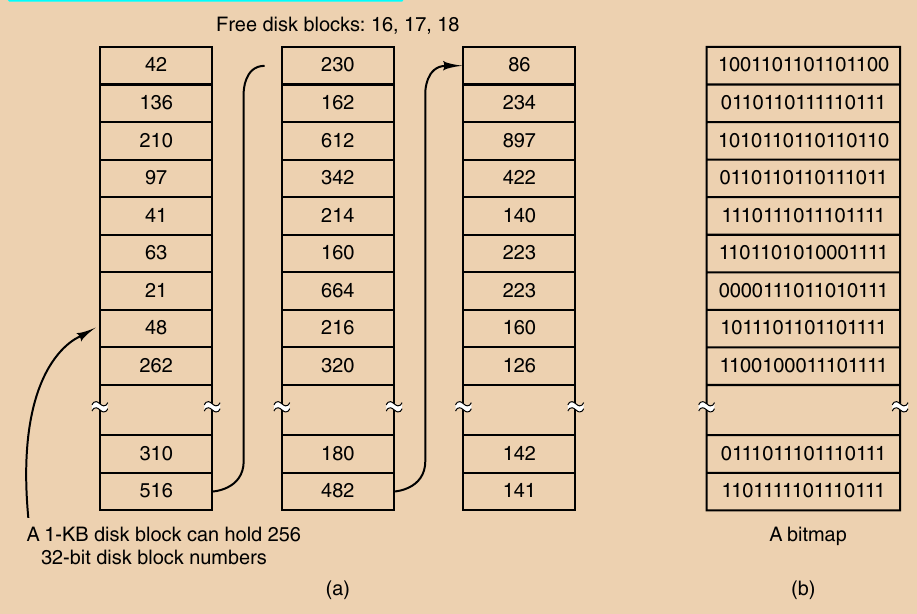
\includegraphics[width=0.45\textwidth]{img/5-18.png}
  \end{center}
  \caption{}
  \label{fig:}
\end{figure}

\subsubsection{Fiabilidade do sistema de arquivos}

A destruição de um sistema de arquivos é muito mais desatrosa do que a destruição de um computador. Se um sistema de arquivos for irrevocavelmente perdido, seja por hardware, software ou ratos nas fitas de backup, restaurar todas as informações será muito difícil e consumirá muito tempo no melhor caso, em muitos será impossível.

Discos rígidos têm blocos ruins desde sua fabricação: é muito caro para o fabricante livrar todos os blocos de defeitos. Uma solução simples de software para blocos ruins existe. Essa solução requer que o usuário ou o sistema de arquivos cuidadosamente contrua um arquivo constituido de todos os blocos ruins. Essa técnica remove eles da lista de blocos livres, para que eles nunca ocorram em arquivos de dados. Se o arquivo de de blocos ruins nunca for lido ou escrito, nenhum problema surgirá. Deve-se ter cuidado durante backups para que esse arquivo não seja lido.

\subsubsection{Backups}

A maioria das pessoas não acham que backups valem a pena, até que em um dia tranquilo seus discos morram abruptamente. 

Backups modernos são geralmente feitos em fitas magnéticas, devido a seu baixo custo por giga armazenado. Fazer backups não é tão trivial e alguns cuidados precisam ser tomados.  

Backups são feitos quando é preciso: recuperar do desastre ou recuperar da estupidez. O primeiro caso é menos comum e ocorre depois de um crash de disco, incêndio, ou outra catástrofe natural. Na prática, essas coisas não acontecem muito frequentemente e é por isso que muitas pessoas não se preocupam com backups. O segundo motivo é quando usuários acidentalmente removem arquivos importantes. Esse problema acontece tão frequentemte que quando um arquivo é "removido" no Windows, ele não é deletado, apenas movido para um diretório especial, a lixeira.

Fazer um backup demora bastante tempo e ocupa um grande quantidade de espaço, por isso, fazer eficientemente e convenientemente é importante.

O primeiro ponto é analisar quais arquivos do sistema de arquivos devem ser incluidos no backup. Certamente, não é necessário incluir todo o sistema de arquivos. Vários programas executáveis podem ser reinstalados a partir de CD-ROMs ou de arquivos fonte, então não precisam ser incluídos. Arquivos temporários não precisam. Em sistemas \unix, todos os arquivos especiais (dispositivos de entrada e saída) são mantidos num diretório /dev. Não só incluir esses arquivos no backup é desnecessário como é perigoso, pois o programa de backup pode rodar indefinidamente se tentar ler por completo esses arquivos. 

Segundo, é desnecessário incluir arquivos que não mudaram desde o último backup: \textbf{backups incrementais}. A forma mais simples de fazer backups incrementais é fazer um backup completo periodicamente, e outros menores diariamente incluindo somente arquivos que mudaram desde o último backup completo (ou diário).

Esse esquema incremental dificulta a restauração. Para recuperar um arquivo, primeiro deve ser restaurado o último backup completo seguido dos backups incrementais em ordem reversa.

Outro problema é que, devido a natureza do processo, grandes quantidades de dados estão presentes nos backups e, por isso, alguma compressão pode ser necessária. Até ai tudo bem, o problema surge quando um único "bad spot" na fita pode invalidar um arquivo inteiro ou até mesmo toda a fita. Portanto, o processo de comprimir o backup deve ser tomado com bastante cuidado.

Uma quarta questão a se considerar é a dificuldade de fazer um backup em um sistema de arquivos ativo. Se arquivos estão sendo modificados durante o backup, o backup resultante pode ser inconsistente. Por essa razão, algoritmos foram escritos para fazer snapshots rápidamente do sistema de arquivos ao copiar estruturas de dados críticas, e então requerir mudanças futuras dos arquivos para copiar os blocos em vez de atualizá-los in place. Dessa forma, o sistema de arquivos é efetivamente congelado no momento do snapshot, para ser feito um backup "sem pressa".

Por último, fazer backups introduz problemas não técnicos. O melhor sistema de segurança online pode ser inútil se o administrador do sistema deixa todas as fitas de backup em seu escritório e o deixa aberto e desprotegido toda vez que caminha até o corredor para pegar um café, por exemplo. Problemas desses tipo devem ser evitados. 

Duas estratégias podem ser feitas para backups em fitas: 

\end{document}


